%\RequirePackage{lineno}

\documentclass[aps,prc,preprint,superscriptaddress,showpacs,showkeys,amsmath]{revtex4-1}
%\documentclass[article,showpacs,preprintnumbers,amsmath,amssymb]{revtex4}
\usepackage{graphicx}
\usepackage[usenames,dvipsnames,svgnames,table]{xcolor}
\usepackage{rotating}
\usepackage{graphicx}% Include  files
\usepackage{dcolumn}% Align table columns on decimal point
\usepackage{bm}% bold math
\usepackage{epsfig}
\usepackage{hyperref}
\usepackage{ulem}

\begin{document}

\newcommand{\Jpsi}{J/\psi}
\newcommand{\pT}{p_{T}}
\newcommand{\calO}{{\cal{O}}}
\newcommand{\barQ}{{\bar{Q}}}
\newcommand{\barq}{{\bar{q}}}
\newcommand{\barc}{{\bar{c}}}
\newcommand{\barb}{{\bar{b}}}
\newcommand{\baru}{\bar{u}}
\newcommand{\barv}{\bar{v}}
\newcommand{\barup}{\bar{u}_{+}}
\newcommand{\barum}{\bar{u}_{-}}
\newcommand{\barvp}{\bar{v}_{+}}
\newcommand{\barvm}{\bar{v}_{-}}
\newcommand{\charm}{{\rm{charm}}}
\newcommand{\bottom}{{\rm{bottom}}}

\newcommand{\cs}{{\hat{s}}}
\newcommand{\ct}{{\hat{t}}}
\newcommand{\cu}{{\hat{u}}}
\newcommand{\alphas}{{\alpha_{s}}}

%\newcommand{}{{}}

\newcommand{\shat}{\hat{\rm s}}
\newcommand{\that}{\hat{\rm t}}
\newcommand{\uhat}{\hat{\rm u}}
\newcommand{\zhat}{\hat{\rm z}}

\newcommand{\CA}{{\cal A}}
\newcommand{\Qbar}{{\overline Q}}
\newcommand{\QQbaroctetgen}{{Q\Qbar[ ^{2S+1}L_J^{(8)}]}}
\newcommand{\QQbaroctetsingS}{{Q\Qbar[ ^1S_0^{(8)}]}}
\newcommand{\QQbaroctettripP}{{Q\Qbar[ ^3P_J^{(8)}]}}
\newcommand{\QQbaroctettripPone}{{Q\Qbar[ ^3P_1^{(8)}]}}

\def\QQbaroctettripS{Q\Qbar[ ^3S_1^{(8)}]}
\def\QQbaroctetPzero{Q\Qbar[ ^3P_0^{(8)}]}
\def\QQbaroctetPone{Q\Qbar[ ^3P_1^{(8)}]}
\def\QQbaroctetPtwo{Q\Qbar[ ^3P_2^{(8)}]}

%\newcommand{\hatt}{\hat{t}}
%\newcommand{\hatu}{\hat{u}}
%\newcommand{\hats}{\hat{s}}


%\linenumbers
\title{{\Large Quarkonia production and dissociation in Pb+Pb collisions}} 
\author{\large Vineet Kumar}
\author{\large Prashant Shukla}
\email{pshukla@barc.gov.in}
\affiliation{Nuclear Physics Division, Bhabha Atomic Research Center, Mumbai, India}
\affiliation{Homi Bhabha National Institute, Anushakti Nagar, Mumbai, India}
%\author{\large Ramona Vogt}
%\affiliation{Nuclear and Chemical Sciences Division, Lawrence Livermore National Laboratory, Livermore, CA 94551, USA}
%\affiliation{Physics Department, University of California, Davis, CA 95616, USA}

\date{\today}

\begin{abstract}
  We calculate the high p$_{T}$ quarkonia production using NRQCD method.
  Different methods of quarkonia suppression are used to explain the high
  p$_{T}$ quarkonia suppression obseved by CMS in LHC
\end{abstract}

\pacs{12.38.Mh, 24.85.+p, 25.75.-q}
\keywords{quark-gluon plasma, quarkonia, suppression, regeneration}

\maketitle

%%%%%%%%%%%%%%%%%%%%%%%%%%%%%%%%%%%%%%%%%%%%%%%%%%%%%%%%%%%%%%%%%%%%%%%%%%%%%%%%%%%%%%%%%%%%%%%%%%%%%%%%%%%%%%%%%

\section{Introduction}

Heavy-ion collisions at relativistic energies are performed to create and characterize 
quark gluon plasma (QGP), a phase of strongly-interacting matter at high energy density 
where quarks and gluons are no longer bound within hadrons.
The quarkonia states ($\Jpsi$ and $\Upsilon$) have been some of the most popular tools 
since their suppression was proposed as a signal of QGP formation \cite{Matsui:1986dk}.
The understanding of these probes has evolved substantially via measurements 
through three generations of experiments: the SPS (at CERN), RHIC (at BNL) and the LHC (at CERN) 
and by a great deal of theoretical activity. (For recent reviews see 
Refs.~\cite{Schukraft:2013wba,Kluberg:2009wc,Brambilla:2010cs}.)
Quarkonia are produced early in the heavy-ion collisions and, if they evolve
through the deconfined medium, their yields should be suppressed in comparison with those in $pp$ collisions. 
The first such measurement was the `anomalous' $\Jpsi$ suppression discovered at the SPS 
which was considered to be a hint of QGP formation. The RHIC measurements showed almost the 
same suppression at a much higher energy contrary to expectation \cite{Brambilla:2010cs,Adare:2011yf}. 
Such an observation was consistent with the scenario that, at higher collision energies, the 
expected greater suppression is compensated by  $\Jpsi$ regeneration through recombination of two 
independently-produced charm quarks~\cite{Andronic:2003zv}. 

In this paper, we calculate $\Jpsi$ and $\Upsilon$ production and
suppression 



%%%%%%%%%%%%%%%%%%%%%%%%%%%%%%%%%%%%%%%%%%%%%%%%%%%%%%%%%%%%%%%%%%%%%%%%%%%%%%%%%%%%%%%
\section{Quarkonia Production in p$+$p collisions}
\label{section:ppProduction}
In this section we describe the production of quarkonia at high transverse
momenta in p$+$p collisions. The factorization formalism of the NRQCD  provides a theoretical 
framework for studying the heavy quarkonium production and decay. 
According to the NRQCD factorization  formalism, the cross-section for direct production of a resonance $H$ in a collision of 
particle $A$ and $B$ can be expressed as 
\begin{equation}
  d\sigma_{A+B\rightarrow H+X} = \sum_{a,b,n}\int dx_a dx_b  G_{a/A}(x_a,\,\mu^{2}_{F}) 
  G_{b/B}(x_b,\,\mu^{2}_{F})\times d\sigma(a+b\rightarrow Q\bar Q(n) +X)<\mathcal{O}^H(n)>
\end{equation}
where, $G_{a/A}(G_{b/B})$ is the parton distribution function (PDF) of the incoming parton $a(b)$ in the incident hadron $A(B)$, which depends on 
the momentum fraction $x_a(x_b)$ and the factorization scale $\mu_F$ as well as on the renormalization scale $\mu_R$. However, 
as we have chosen $\mu_F$ = $\mu_R$, in our case PDFs are function of $x$ and $\mu_F$ only. The tranverse mass of the 
resonance $H$ is $m_T = \sqrt{p_T^2 + m_H^2}$, where $m_H\sim2m_Q$ is the mass of resonance $H$. The short distance 
contribution $d\sigma(a+b\rightarrow Q\bar Q(n) +X)$ can be calculated within the framework of perturbative QCD (pQCD). 
On the other hand, $<\mathcal{O}^H(n)>$ (the state $n=^{2S+1}L^{[i]}_J$) are nonperturbative LDMEs and can be estimated on the basis of 
the comparison with experimental measurements. 

The dominant processes in evaluating the differential 
yields of heavy mesons as a function of $p_T$ are the $2\rightarrow 2$
processes of the kind $g+q\rightarrow H+q$, $q+\bar{q}\rightarrow H+g$ and
$g+g\rightarrow H+g$, where $H$ refers to the heavy meson. We label the process
generically as $a+b\rightarrow c+d$, where $a$ and $b$ are light incident
partons, $c$ refers to $H$ and $d$ is a light final-state parton. The differential cross-section 
for the short distance contribution i.e. the heavy quark pair production 
from the reaction of the type $a\,+\,b\,\rightarrow\,c\,+\,d$ can be written as~\cite{Owens:1986mp}

\begin{equation}
  \frac{{d\sigma}^{ab\rightarrow cd}}{dp_T\,dy} = \int dx_a\, G_{a/A}(x_a,\,\mu^{2}_{F})\, G_{b/B}(x_b,\,\mu^{2}_{F})\times 
  2p_T \frac{x_a\,x_b}{x_a-\frac{m_T}{\sqrt{s}}e^y}\frac{d\sigma}{d\hat t}(ab\rightarrow cd),
\end{equation}

where, $\sqrt{s}$ being the total energy in the centre-of-mass and $y$ is the rapidity of 
the $Q\bar Q$ pair. In our numerical computation, we use CTEQ6M~\cite{Lai:2010vv} for the parton 
distribution functions. The invariant differential cross-section is given by
\begin{equation}
\frac{d\sigma}{d\hat t} = \frac{|\mathcal{M}|^2}{16\pi{\hat s}^2},
\end{equation}
where $\hat s$ and $\hat t$ are the parton level Mandelstam variables. $\mathcal{M}$ is the 
feynman amplitude for the process. Energy momentum conservation fixes value of the momentum 
fraction $x_b$ as,
\begin{equation}
x_b = \frac{1}{\sqrt{s}}\frac{x_a\,\sqrt{s}\,m_T\,e^{-y}-m^2_H}{x_a\,\sqrt{s}-m_T\,e^y}.
\end{equation}

The minimum value of $x_a$ is 
\begin{equation}
x_{a\rm min} = \frac{1}{\sqrt{s}}\frac{\sqrt{s}\,m_T\,e^{y}-m^2_H}{\sqrt{s}-m_T\,e^{-y}}.
\end{equation}

\begin{figure}
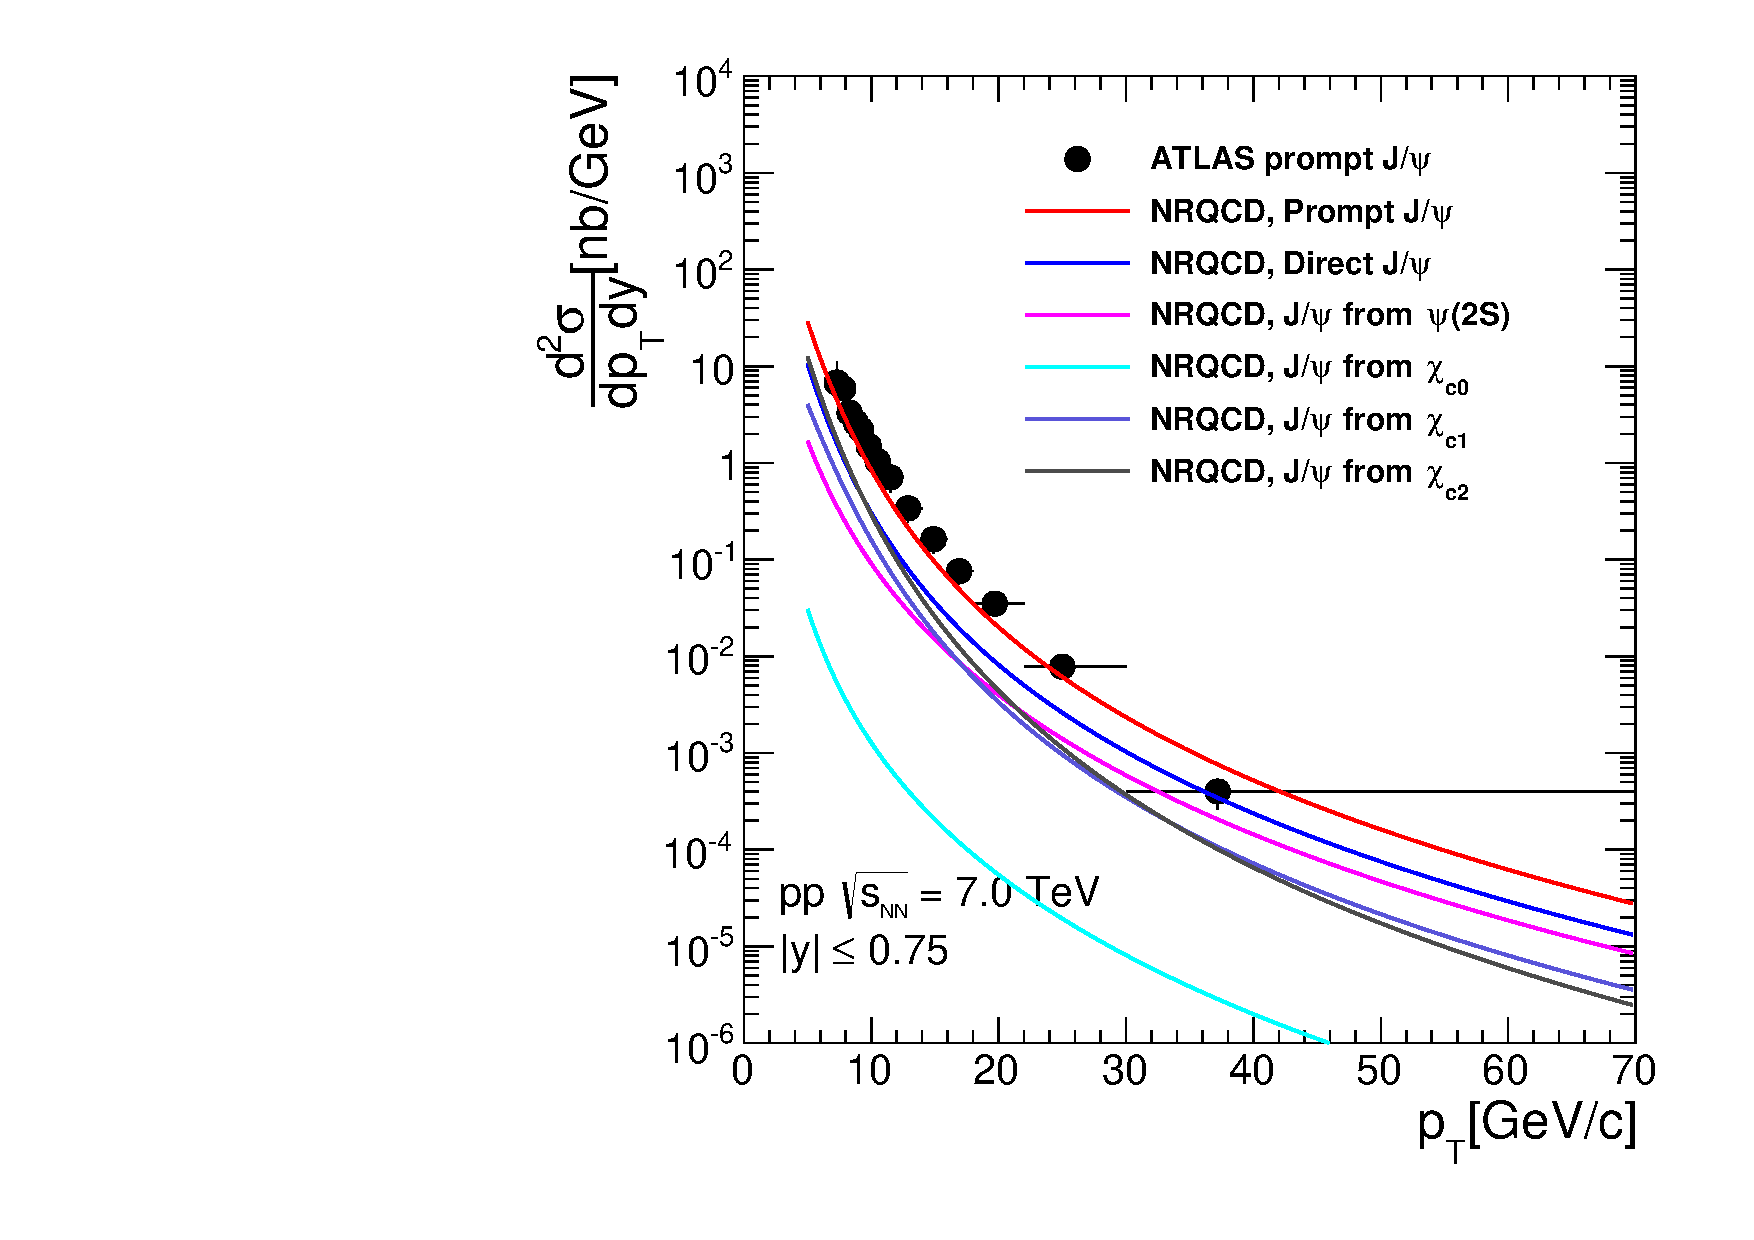
\includegraphics[width=0.49\textwidth]{Fig1b_JPsi_ATLAS_Y075_S7TeV.pdf}
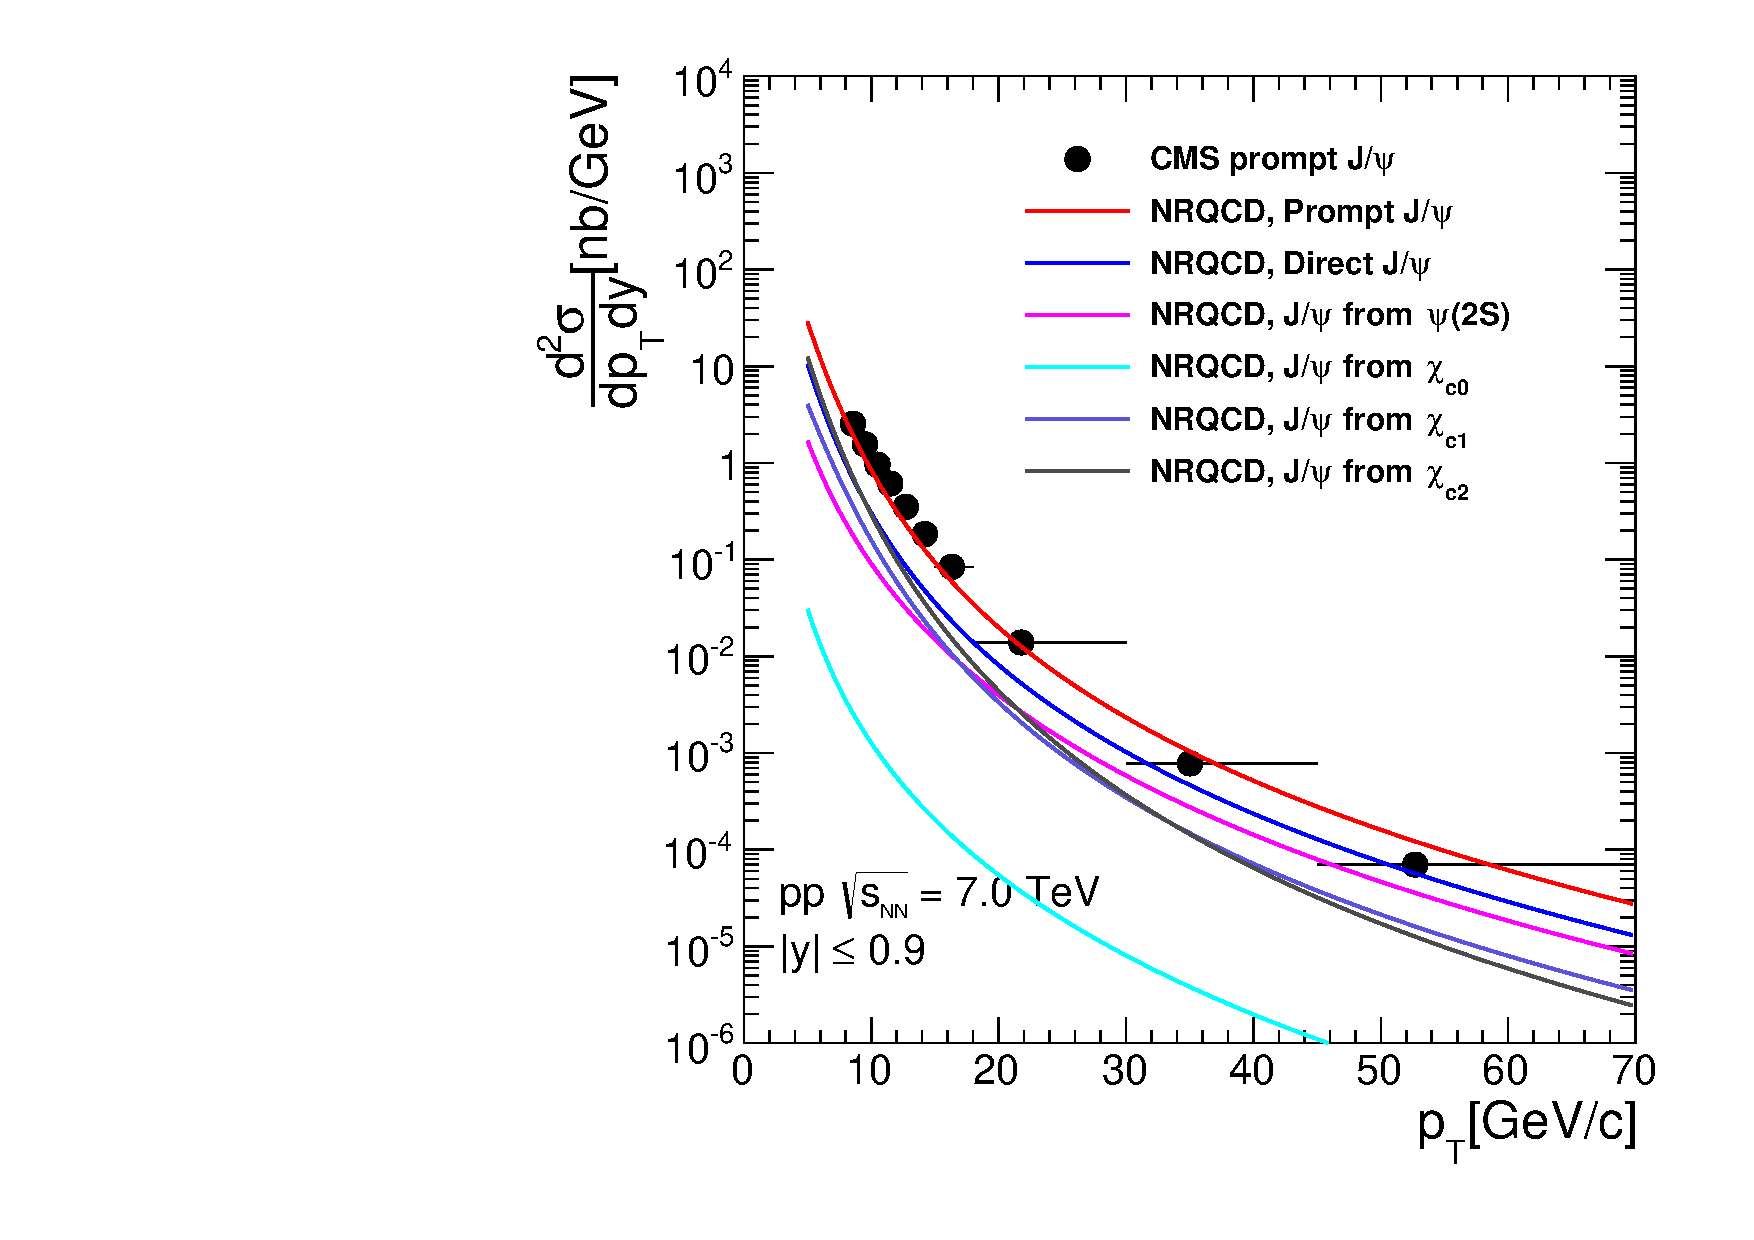
\includegraphics[width=0.49\textwidth]{Fig1a_JPsi_CMS_Y090_S7TeV.pdf}
\caption{(Color online) Differential production cross-section of $J/\psi$ as a function of $p_{T}$ compared 
  with the ATLAS~\cite{Aad:2011sp} and CMS~\cite{Chatrchyan:2011kc} data.}
\label{fig:TauVsTemp}
\end{figure}


The LDMEs are predicted to scale with a definite power of the relative velocity $v$ of the heavy constituents inside $Q\bar Q$ bound states. 
In the limit $v<<1$, the production of quarkonium is based on the $^3S_1^{[1]}$ and $^3P_J^{[1]}$ ($J$ = 0,1,2) CS states 
and $^1S_0^{[8]}$, $^3S_1^{[8]}$ and $^3P_J^{[8]}$ CO states. In our calculations, we used the expressions for the short distance CS cross-sections 
given in Refs.~\cite{Baier:1983va,Humpert:1986cy,Gastmans:1987be} and the CO cross-sections given in Refs.~\cite{Cho:1995vh,Cho:1995ce}.

In this section we calculate the $p_T$ distribution of $J/\psi$, $\psi(2S)$ and $\Upsilon$(nS) mesons in $p-p$ collisions 
at LHC energies. For $J/\psi$ production in $p-p$ collisions, three sources need to be considered: 
direct $J/\psi$ production, feed-down contributions to the $J/\psi$ from the decay of heavier charmonium states, 
predominantly from $\psi(2S)$, $\chi_{c0}$, $\chi_{c1}$ and $\chi_{c2}$ and $J/\psi$ 
from $B$ hadron decays. The sum of the first two sources is called "prompt $J/\psi$" and the third source will be called "$J/\psi$ from $B$". 
On the other hand, $\psi(2S)$ has no significant feed-down contributions from higher mass states. We call this direct contribution as 
"prompt $\psi(2S)$" to be consistent with the experiments. The other source to $\psi(2S)$ production is from $B$ hadron decays and
 we call it "$\psi(2S)$ from $B$". The sum of the prompt $J/\psi$($\psi(2S)$) and $J/\psi$($\psi(2S)$) from $B$ will be called 
"inclusive $J/\psi$($\psi(2S)$)". Similar terminology is used for $\Upsilon$ states, only differnce is that we do not have 
any contribution from open T mesons.

NRQCD provides a systematic procedure to compute any quantity as an expansion in the relative velocity $v$
of the heavy quarks in the meson. For example, the wavefunction of the $J/\psi$
meson (analogous expressions hold for the $\psi(2S)$, $\Upsilon(1S)$,
$\Upsilon(2S)$ and $\Upsilon(3S)$) is written as

\begin{equation}
\begin{split}
|J/\psi\rangle = &|Q\barQ([^3S_1]_{1})\rangle 
+ \calO(v)|Q\barQ([^1S_0]_{8}g)\rangle 
  + \calO(v^2)|Q\barQ([^3S_1]_{8}gg)\rangle\\
  &+ \calO(v^1)|Q\barQ([^3P_0]_{8}g)\rangle
  + \calO(v^1)|Q\barQ([^3P_1]_{8}g)\rangle
  + \calO(v^1)|Q\barQ([^3P_2]_{8}g)\rangle
  +\cdot\cdot\cdot
  \label{eq:Jfock}
\end{split}
\end{equation}

The differential cross section for the direct production of $J/\psi$ can be written 
as the sum of the contributions,
\begin{equation}
\begin{split}
d\sigma(J/\psi) &= d\sigma(Q\barQ([^3S_1]_{1}))
                  \langle \calO(Q\barQ([^3S_1]_{1})\rightarrow J/\psi)\rangle 
                +  d\sigma(Q\barQ([^1S_0]_{8}))
                  \langle \calO(Q\barQ([^1S_0]_{8})\rightarrow J/\psi)\rangle\\ 
                &+  d\sigma(Q\barQ([^3S_1]_{8}))
                  \langle \calO(Q\barQ([^3S_1]_{8})\rightarrow J/\psi)\rangle 
                +  d\sigma(Q\barQ([^3P_0]_{8}))
                  \langle \calO(Q\barQ([^3P_0]_{8})\rightarrow J/\psi)\rangle\\ 
                &+  d\sigma(Q\barQ([^3P_1]_{8}))
                  \langle \calO(Q\barQ([^3P_1]_{8})\rightarrow J/\psi)\rangle
                +  d\sigma(Q\barQ([^3P_2]_{8}))
                  \langle \calO(Q\barQ([^3P_2]_{8})\rightarrow J/\psi)\rangle
                + \cdot\cdot\cdot  \;,
\label{eq:dsigmaJ}
\end{split}
\end{equation}
where the quantity in the brackets $[\;]$ represents the angular momentum
quantum numbers of the $Q\barQ$ pair in the Fock expansion. The subscript on
$[\;]$ refers to the color structure of the $Q\barQ$ pair, $1$ being 
the color-singlet and $8$ being the color-octet. The dots represent terms which contribute at
higher powers of $v$. The short distance cross sections $d\sigma(Q\barQ)$
correspond to the production of a $Q\barQ$ pair in a particular color and spin
configuration, while the long distance matrix element
$\langle\calO(Q\barQ)\rightarrow J/\psi\rangle$ corresponds to the probability
of the $Q\barQ$ state to convert to the quarkonium wavefunction. This
probability includes any necessary prompt emission of soft gluons to prepare a
color neutral system that matches onto the corresponding Fock component of the
quarkonium wavefunction. 


Power counting rules tell us that contributions from the color-octet matrix
elements in Eq.~\ref{eq:dsigmaJ} are suppressed by $v^4$ compared to the color
singlet matrix elements. More specifically,
\begin{equation}
\begin{split}
\langle \calO(Q\barQ([^3S_1]_{1})\rightarrow J/\psi)\rangle &= \calO(m_Q^3 v^3)\;, \\
\langle \calO(Q\barQ([^3S_1]_{8})\rightarrow J/\psi)\rangle &= \calO(m_Q^3 v^7)\;, \\
\langle \calO(Q\barQ([^1S_0]_{8})\rightarrow J/\psi)\rangle &= \calO(m_Q^3 v^7)\;, \\
\langle \calO(Q\barQ([^3P_J]_{8})\rightarrow J/\psi)\rangle &= 
\calO(m_Q^5 v^7) \;. ~\label{eq:scalingsJ}
\end{split}
\end{equation}
These operators are multiplied by the short distance differential cross sections,
which are related to the probability to create $Q\barQ$ pairs in specific
quantum states. Since these are short distance operators, they can be
calculated in perturbation theory. We use the expressions for the short
distance color-singlet cross sections given in~\cite{Baier:1983va, Humpert:1986cy} 
and the color-octet cross sections given in~\cite{Cho:1995ce,Cho:1995vh,Braaten:2000cm}.

The case of the $p$-wave bound states ($\chi_{c0}$, $\chi_{c1}$, and
$\chi_{c2}$, sometimes collectively referred to as $\chi_{cJ}$, and the
corresponding states of the $b$ quark) is slightly
different. The wavefunction of $\chi_c$ states can be written as
\begin{equation}
\begin{split}
|\chi_{cJ}\rangle = & |Q\barQ([^3P_J]_{1})\rangle 
  + \calO(v)|Q\barQ([^3S_1]_{8}g)\rangle
  + \calO(v^2)|Q\barQ([^1S_0]_{8}g)\rangle
  + \calO(v)|Q\barQ([^3D_J]_{8}g)\rangle\\
  &+ \calO(v^2)|Q\barQ([^1P_1]_{8}g)\rangle
  + \calO(v^2)|Q\barQ([^3P_J]_{8}gg)\rangle
  +\cdot\cdot\cdot
  \label{eq:chifock}
\end{split}
\end{equation}
The color-singlet state $Q\barQ[^3P_J]_{1}$ and the color-octet state
$Q\barQ[^3S_1]_{8}$ contribute to the same order in $v$ because of the angular
momentum barrier for $p-$wave states, and hence both need to be included for a consistent
calculation in $v$.  For the calculation of the production cross section, we
consistently take the contributions to the lowest order in $v$.
For example the $\chi_{c}$ contribution is
\begin{equation}
\begin{split}
d\sigma(\chi_{cJ}) &= d\sigma(Q\barQ([^3P_J]_{1}))
                  \langle \calO(Q\barQ([^3P_J]_{1})\rightarrow \chi_{cJ})\rangle 
                +  d\sigma(Q\barQ([^3S_1]_{8}))
                  \langle \calO(Q\barQ([^3S_1]_{8})\rightarrow \chi_{cJ})\rangle
                + \cdot\cdot\cdot  
\label{eq:dsigmachi}
\end{split}
\end{equation}
Similar expressions hold for the $\chi_b(1P), \chi_b(2P)$ and $\chi_b(3P)$ 
mesons. The expressions for the short distance coefficients are given
in~\cite{Cho:1995vh}. The scaling of the matrix elements is given as
\begin{equation}
\begin{split}
\langle \calO(Q\barQ([^3P_J]_{1})\rightarrow \chi_{cJ})\rangle &= 
\calO(m_Q^5 v^5) \;,\\
\langle \calO(Q\barQ([^3S_1]_{8})\rightarrow \chi_{cJ})\rangle &= 
\calO(m_Q^5 v^5)\;.~\label{eq:scalingschi}
\end{split}
\end{equation}

Therefore we need the color-singlet and color-octet matrix elements
to obtain theoretical results for the production of quarkonia at RHIC and
LHC energies.


\subsection{Feed-down contributions}

For the net production of $J/\psi$ we consider the direct contribution, and
feed-down contributions from $\chi_{c0}(1P)$, $\chi_{c1}(1P)$,
$\chi_{c2}(1P)$ and $\psi(2S)$. The relevant branching fractions are given
in Table~\ref{table:CharmoniaBFs},

\begin{table*}[h]
\begin{tabular}{c|cccc}
meson from &to $\chi_{c0}$ &to $\chi_{c1}$ &to $\chi_{c2}$ &to $J/\psi$\\ 
\hline
$\psi(2S)$ & 0.0962 & 0.092 & 0.0874 & 0.595   \\
$\chi_{c0}$& &  &  & 0.0116           \\
$\chi_{c1}$& &  &  & 0.344           \\
$\chi_{c2}$& &  &  & 0.195           \\
\end{tabular}
\caption{Relevant branching fractions for charmonia~\cite{Nakamura:2010zzi}}
\label{table:CharmoniaBFs}
\end{table*}

$B$ hadrons can also decay to $J/\psi$($\psi$(2S)) with a net effective branching fraction
$B(H_b\rightarrow J/\psi+X)_{\rm {eff}} =1.16(2.83)\times10^{-2}$~\cite{Acosta:2004yw}. 
In particular, at high $p_T$, the contribution to the inclusive yield from the decay of $B-$hadrons is
substantial, and can possibly even dominate production.

The analysis of $\Upsilon$(1S) production and feed-down contributions is very
similar to the analysis for J/$\psi$. Following~\cite{Cho:1995ce,Cho:1995vh}
we consider states up to $n=3$. For the $\Upsilon$(3S), we consider only the
direct contribution. For $\Upsilon$(2S), we consider feed-down from
$\Upsilon$(2S) and $\chi_b$(2P). For $\Upsilon$(1S) there are additional
contributions from $\Upsilon$(2S) and $\chi_b$(1P). The relevant branching
fractions are given in Table~\ref{table:BottomoniaBFs}.

\begin{table*}[h]
\begin{tabular}{c|cccccccc}
meson from  &to $\chi_{b0}(2)$ &to $\chi_{b1}(2)$ &to $\chi_{b2}(2)$
            &to $\Upsilon(2S)$
            &to $\chi_{b0}(1)$ &to $\chi_{b1}(1)$ &to $\chi_{b2}(1)$ 
            &to $\Upsilon(1S)$\\ 
\hline
$\Upsilon(3S)$ & 0.131 & 0.126 & 0.059 
               & 0.199
               & 0.003 & 0.0017 & 0.019
               & 0.066\\
$\chi_{b0}(2P)$& & &
               & 0.046
               & & &
               & 0.009\\
$\chi_{b1}(2P)$& & &
               & 0.21
               & & &
               & 0.101\\
$\chi_{b2}(2P)$& & &  
               & 0.162
               & & &
               & 0.082\\
$\Upsilon(2S)$ & & &
               &
               & 0.038 & 0.0715 & 0.069 
               & 0.267\\
$\chi_{b0}(1P)$& & &  
               &
               & & &
               & 0.06\\
$\chi_{b1}(1P)$& & &
               &
               & & &
               & 0.35\\
$\chi_{b2}(1P)$& & &
               &
               & & &
               & 0.22\\
\end{tabular}
\caption{Relevant branching fractions for bottomonia~\cite{Nakamura:2010zzi}}
\label{table:BottomoniaBFs}
\end{table*}


\subsection{Long distance matrix elements (LDME) for quarkonia production}
\label{section:Matrix}

\subsubsection{Color Singlet Matrix elements}

In this work, following~\cite{Cho:1995ce,Cho:1995vh} we use the values of the
color-singlet operators calculated using the potential model. The expressions
and the values for the color-singlet operators are given
in~\cite{Cho:1995ce,Cho:1995vh,Eichten:1994gt}. The values are obtained by
solving the non-relativistic wavefunctions:
\begin{equation}
\begin{split}
\begin{array}{ccc}
\langle \calO(c\barc([^3S_1]_{1})\rightarrow J/\psi)\rangle 
=3\langle \calO(c\barc([^1S_0]_{1})\rightarrow J/\psi)\rangle
&=3N_c\frac{|R_{n=1}(0)|^2}{2\pi}
&=1.2\;{\rm GeV^3} \;, \\
\langle \calO(c\barc([^3S_1]_{1})\rightarrow \psi(2S))\rangle 
=3\langle \calO(c\barc([^1S_0]_{1})\rightarrow \psi(2S))\rangle
&=3N_c\frac{|R_{n=2}(0)|^2}{2\pi}
&=0.76\;{\rm GeV^3} \;, \\
\frac{1}{5}\langle \calO(c\barc([^3P_2]_{1})\rightarrow \chi_{c2}(1P))\rangle
=\frac{1}{3}\langle \calO(c\barc([^3P_1]_{1})\rightarrow \chi_{c1}(1P))\rangle 
=&&\\ 
\langle \calO(c\barc([^3P_0]_{1})\rightarrow \chi_{c0}(1P))\rangle 
&=3N_c\frac{|R^\prime_{n=1}(0)|^2}{2\pi}
&=0.054 m_{\charm}^2\;{\rm GeV^3}\; ,
\end{array}
\label{eq:charmsinglet}
\end{split}
\end{equation}

where $R(0)$ is the radial wavefunction at the origin, $R^\prime(0)$ is the
first derivative of the radial wavefunction at the origin, and $n$ refers to
the radial quantum number. We take the mass of the charm quark,
$m_{\charm}=1.4$GeV. 

The values of the color-singlet operators for  bottomonia are given
in~\cite{Braaten:2000cm}, which we reproduce here:
\begin{equation}
\begin{split}
\begin{array}{ccc}
\langle \calO(b\barb([^3S_1]_{1})\rightarrow \Upsilon(1S))\rangle &=
3N_c\frac{|R_{n=1}(0)|^2}{2\pi}
&=10.9\;{\rm GeV^3} \;, \\
\langle \calO(b\barb([^3P_0]_{1})\rightarrow \chi_{b0}(1P))\rangle &= 
3N_c\frac{|R^\prime_{n=1}(0)|^2}{2\pi}
&=0.100 m_{\bottom}^2\;{\rm GeV^3}\;, \\
\langle \calO(b\barb([^3S_1]_{1})\rightarrow \Upsilon(2S))\rangle &=
3N_c\frac{|R_{n=2}(0)|^2}{2\pi}
&=4.5\;{\rm GeV^3}\;, \\
\langle \calO(b\barb([^3P_0]_{1})\rightarrow \chi_{b0}(2P))\rangle &= 
3N_c\frac{|R^\prime_{n=2}(0)|^2}{2\pi}
&=0.036 m_{\bottom}^2 \;{\rm GeV^3} \;, \\
\langle \calO(b\barb([^3S_1]_{1})\rightarrow \Upsilon(3S))\rangle &=
3N_c\frac{|R_{n=3}(0)|^2}{2\pi}
&=4.3\;{\rm GeV^3} \; ,
\end{array}
\label{eq:bottomsinglet}
\end{split}
\end{equation}
where we use $m_{\bottom}=4.88$GeV~\cite{Cho:1995ce,Cho:1995vh}.



\subsubsection{Color Octet Matrix elements}
The color-octet operators can not be related to the non-relativistic
wavefunctions of $Q\barQ$ since it involves a higher Fock state.
We used following values for Color Octet Matrix elements as given in Ref.~\cite{Sharma:2012dy}.
%Following~\cite{Cho:1995ce,Cho:1995vh,Braaten:2000cm}, we fit them to the data.
\begin{equation}
\begin{split}
\langle \calO(c\barc([^3S_1]_{8})\rightarrow J/\psi)\rangle
&=(0.0013\pm0.0013)\;{\rm GeV^3} \;, \\
\langle \calO(c\barc([^1S_0]_{8})\rightarrow J/\psi)\rangle 
&=(0.018\pm0.0087)\;{\rm GeV^3}\;, \\
&=\langle \calO(c\barc([^3P_0]_{8})\rightarrow J/\psi)\rangle/(m_{\charm}^2) 
\;, \\
\langle \calO(c\barc([^3S_1]_{8})\rightarrow \psi(2S))\rangle
&=(0.0033\pm0.00021)\;{\rm GeV^3} \;, \\
\langle \calO(c\barc([^1S_0]_{8})\rightarrow \psi(2S))\rangle 
&=(0.0080\pm0.00067)\;{\rm GeV^3}\;, \\
&=\langle \calO(c\barc([^3P_0]_{8})\rightarrow J/\psi)\rangle/(m_{\charm}^2) 
\;, \\
\langle \calO(c\barc([^3P_1]_{8})\rightarrow J/\psi)\rangle 
&=3\times\langle \calO(c\barc([^3P_0]_{8})\rightarrow J/\psi)\rangle \;, \\
\langle \calO(c\barc([^3P_2]_{8})\rightarrow J/\psi)\rangle 
&=5\times\langle \calO(c\barc([^3P_0]_{8})\rightarrow J/\psi)\rangle\;, \\
\langle \calO(c\barc([^3S_1]_{8})\rightarrow \chi_{c0}(1P))\rangle 
&=(0.00187\pm0.00025)\;{\rm GeV^3}\;, \\
\label{eq:charmoctet} \;.
\end{split}
\end{equation}
Since the shape of the short distance part as a function of $p_T$ is very
similar for $[^1S_0]_8$ and $[^3P_0]_8$ contributions~\cite{Cho:1995ce,Cho:1995vh}, 
only fit a linear combination of these elements is fitted.

The octet matrix elements for the bottomonia are obtained by fitting
TeVatron~\cite{Acosta:2001gv} and the LHC~\cite{Khachatryan:2010zg} data
and are as follows:
\begin{equation}
\begin{split}
\langle \calO(b\barb([^3S_1]_{8})\rightarrow \Upsilon(1S))\rangle
&=(0.0477\pm0.0334)\;{\rm GeV^3} \;,\\
\langle \calO(b\barb([^1S_0]_{8})\rightarrow \Upsilon(1S))\rangle
&=(0.0121\pm0.040)\;{\rm GeV^3}\;, \\
&=\langle \calO(b\barb([3P_0]_{8})\rightarrow \Upsilon(1S))\rangle
/(5m_{\bottom}^2) \;, \\
\langle \calO(b\barb([^3S_1]_{8})\rightarrow \chi_{b0}(1P))\rangle
&=(0.1008)\;{\rm GeV^3}\;, \\
\langle \calO(b\barb([^3S_1]_{8})\rightarrow \Upsilon(2S))\rangle
&=(0.0224\pm0.02)\;{\rm GeV^3}\;, \\
\langle \calO(b\barb([^1S_0]_{8})\rightarrow \Upsilon(2S))\rangle
&=(-0.0067\pm0.0084)\;{\rm GeV^3}\;, \\
&=\langle \calO(b\barb([3P_0]_{8})\rightarrow \Upsilon(2S))\rangle
/(5m_{\bottom}^2)\\
\langle \calO(b\barb([^3S_1]_{8})\rightarrow \chi_{b0}(2P))\rangle
&=(0.0324)\;{\rm GeV^3}\; ,\\
\langle \calO(b\barb([^3S_1]_{8})\rightarrow \Upsilon(3S))\rangle
&=(0.0513\pm0.0085)\;{\rm GeV^3}\;, \\
\langle \calO(b\barb([^1S_0]_{8})\rightarrow \Upsilon(3S))\rangle
&=(0.0002\pm0.0062)\;{\rm GeV^3}\;, \\
&=\langle \calO(b\barb([3P_0]_{8})\rightarrow \Upsilon(3S))\rangle
/(5m_{\bottom}^2)
\label{eq:bottomoctet}
\end{split}
\end{equation}

For a more sophisticated fitting of the color-octet matrix elements including
NLO effects, see~\cite{Butenschoen:2010rq, Butenschoen:Long,
Butenschoen:polarised}.

\subsection{Short distance pQCD cross sections for quarkonia production}
\label{section:pqcd}

Here we list the lowest order QCD cross sections for the resonance production used 
in our calculations. We write the formulas in terms of the invariants $\cs$,$\ct$,$\cu$.
where $\cs^2 + \ct^2 + \cu^2 = M^2$ and $M$ is the mass of the resonance considered.
These parton level invariants are related with the rapidity,y 
and transeverse momentum $p_{T}$ of the resonance with following relations

\begin{equation}
\begin{split}
\cs = \,&x_{a}\,x_{b}\,s \\
\ct = \,&M^{2} - x_{a}\,\sqrt{s}\,m_{T}\,e^{-y}\\
\cu = \,&M^{2} - x_{b}\,\sqrt{s}\,m_{T}\,e^{y}\\
 \end{split}  
\end{equation}

The subprocesses of resonance production can be
grouped as follows.

 To order $\alpha_{s}^{2}$ one only has the
gluon fusion processes, g g $\rightarrow ^{(2S+1)}L_{J}$. This 
process gives resonance with very small $\pT$, so we do not 
use these corss sections in our calculations.

To order $\alpha_{s}^{3}$, on the other hand, one has typically
two-by-two scattering processes. The relevant cross
sections are given below:
\subsubsection{Color Singlet PQCD cross sections}
\begin{itemize}
\item g q $\rightarrow {\rm ^{(2S+1)}L_{J}}$ q or (q$\rightarrow \bar{\rm q})$
\begin{equation}
\begin{split}
\frac{d\sigma}{d\ct}(^1S_0) = &\frac{2\pi\alphas^{3} (R_{0})^{2}}{9M\cs^2}\cdot\frac{(\ct-M^2)^{2}-2\cs\cu}{(-\ct)(\ct-M^2)^{2}}\\
\frac{d\sigma}{d\ct}(^3P_0) = &\frac{8\pi\alphas^3 (R_{1}^\prime)^{2}}{9M^{3}\cs^2}\cdot\frac{(\ct-3M^2)^{2}(\cs^2+\cu^2)}{(-\ct)(\ct-M^2)^{4}}\\
\frac{d\sigma}{d\ct}(^3P_1) = &\frac{16\pi\alphas^3 (R_{1}^\prime)^{2}}{3M^{3}\cs^2}\cdot\frac{-\ct(\cs^2+\cu^2)-4M^2\cs\cu}{(\ct-M^2)^{4}}\\
\frac{d\sigma}{d\ct}(^3P_2) = &\frac{16\pi\alphas^3 (R_{1}^\prime)^{2}}{9M^{3}\cs^2} \cdot \\
                              &\frac{(\ct-M^2)^2(\ct^2+6M^4)-2\cs\cu(\ct^2-6M^2(\ct-M^2))}{(-\ct)(\ct-M^2)^4}\\
\end{split}  
\end{equation}
\item q $\bar{\rm q}$ $\rightarrow {\rm ^{(2S+1)}L_{J}}$ g
\begin{equation}
\frac{d\sigma}{d\ct}({\rm ^{(2S+1)}L_{J}})=-\frac{8}{3}\frac{\ct^2}{\cs^2}\frac{d\sigma}{d\ct}({\rm g q \rightarrow ^{(2S+1)}L_{J} q})|_{\ct\leftrightarrow\cu}
\end{equation}
\item g g $\rightarrow {\rm ^{(2S+1)}L_{J}}$ g
\begin{equation}
\begin{split}
\frac{d\sigma}{d\ct}(^3S_1) = &\frac{5\pi\alphas^{3} (R_{0})^{2}}{9M\cs^2}\cdot \frac{M^2}{(\cs-M^2)^2 (\ct-M^2)^2 (\cu-M^2)^2}\\
                             &\cdot \{[\cs^2(\cs-M^2)^2]+[\cs\rightarrow\ct]+[\cs\rightarrow\cu] \}\\
\frac{d\sigma}{d\ct}(^1S_0) = &\frac{\pi\alphas^{3} (R_{0})^{2}}{2M\cs^2}\frac{1}{\cs\ct\cu(\cs-M^2)^2(\ct-M^2)^2(\cu-M^2)^2}\\
                              &\cdot\{[\cs^4(\cs-M^2)^2((\cs-M^2)^2+2M^4)\\
                              &-\frac{4}{3}\cs\ct\cu(\cs^2+\ct^2+\cu^2)(\cs-M^2)(\ct-M^2)(\cu-M^2)\\
                              &+\frac{16}{3}M^2\cs\ct\cu(\cs^2\ct^2+\cs^2\cu^2+\ct^2\cu^2)\\
                              &+\frac{28}{3}M^4\cs^2\ct^2\cu^2]+[\cs\leftrightarrow\ct]+[\cs\leftrightarrow\cu]\}\\
\end{split}  
\end{equation}
We define two new variables as a combination of $\cs,\ct and \cu$. These variables can  be used to define 
the g g $\rightarrow {\rm ^{(2S+1)}L_{J}}$ g cross sections.
cross sections
\begin{equation}
\begin{split}
  P = & \,\cs\ct + \ct\cu + \cu\cs \\
  Q = & \,\cs\ct\cu\\
\end{split} 
\end{equation}
\begin{equation}
\begin{split}
\frac{d\sigma}{d\ct}(^1S_0) = ~&\frac{\pi \alphas^3 (R_{0})^{2}}{M\cs^2}\frac{P^2(M^8-2M^4P+P^2+2M^2Q)}{Q(Q-M^2P)^2}\\
\frac{d\sigma}{d\ct}(^3S_1) = ~&\frac{10\pi \alphas^3 (R_{0})^{2}}{9\cs^2}\frac{M(P^2-M^2Q)}{(Q-M^2P)^2}\\
\frac{d\sigma}{d\ct}(^1P_1) = ~&\frac{40\pi \alphas^3 (R_{1}^\prime)^{2}}{3M\cs^2}\frac{[-M^{10}P + M^6P^2 + Q(5M^8-7M^4P+2P^2)+4M^2Q^2]}{(Q-M^2P)^3}\\
\frac{d\sigma}{d\ct}(^3P_0) = ~&\frac{4\pi \alphas^3 (R_{1}^\prime)^{2}}{M^3\cs^2}\frac{1}{Q(Q-M^2P)^4}[9M^4P^4(M^8-2M^4P+P^2)\\
                              ~&-6M^2P^3Q(2M^8-5M^4P+P^2)\\
                              ~&-P^2Q^2(M^8+2M^4P-P^2)\\
                              ~&+2M^2PQ^3(M^4-P)+6M^4Q^4]\\
\frac{d\sigma}{d\ct}(^3P_1) = ~&\frac{12\pi \alphas^3 (R_{1}^\prime)^{2}}{M^3\cs^2}\frac{P^2\{M^2P^2(M^4-4P)-2Q(M^8-5M^4P-P^2)-15M^2Q^2\}}{(Q-M^2P)^4}\\
\frac{d\sigma}{d\ct}(^3P_2) = ~&\frac{4\pi \alphas^3 (R_{1}^\prime)^{2}}{M^3\cs^2}\frac{1}{Q(Q-M^2P)^4}\\
                             ~&\{12M^4P^4(M^8-2M^4P+P^2) - 3M^2P^3Q(8M^8-M^4P+4P^2)\\
                             ~&-2P^2Q^2(7M^8-43M^4P-P^2)+M^2PQ^3(16M^4-61P)\\
                             ~&+12M^4Q^4\}\\
\end{split}  
\end{equation}
\end{itemize}



\subsubsection{Color Octet PQCD cross sections}
We list below short distance squared amplitudes for $2 \to 2$ scattering 
processes which mediate color-octet quarkonia production. 
These expressions are averaged over initial spins and colors of the two 
incident partons.  The helicity levels of outgoing $J=1$ and $J=2$ pairs 
are labeled by the subscript $h$.  The total squared amplitudes for creating 
specific quarkonia states can be obtained by multiplying these process-independent 
short distance expressions with appropriate long distance NRQCD matrix 
elements. 


\bigskip


\begin{itemize}
\item q $\bar{\rm q}$ $\rightarrow Q\barQ[{\rm ^{(2S+1)}L_{J}^{(8)}}]$ g

\begin{equation}
\begin{split}
%{\overline{\sum}} | \CA(q\barq \to \QQbaroctetsingS g) |^2 &= {5 (4\pi \alphas)^3 \over 27 M} {\ct^2+\cu^2 \over \cs (\cs-M^2)^2}\\
\mathop{{\bar{\sum}}} | \CA(q\barq \to \QQbaroctetsingS g) |^2 &= {5 (4\pi \alphas)^3 \over 27 M} {\ct^2+\cu^2 \over \cs (\cs-M^2)^2}\\
\mathop{{\bar{\sum_{h=0}}}} | \CA(q\barq \to \QQbaroctettripS g) |^2 &= {8 (4\pi \alphas)^3 \over 81 M^3} {M^2 \shat \over (\shat-M^2)^4} 
\bigl[4(\that^2+\uhat^2)-\that\uhat \bigr]\\
\mathop{{\bar{\sum_{|h|=1}}}} | \CA(q\barq \to \QQbaroctettripS g) |^2 &= {2 (4\pi \alphas)^3 \over 81 M^3} {\shat^2+M^4 \over (\shat-M^2)^4} 
{\that^2+\uhat^2 \over \that\uhat} \bigl[4(\that^2+\uhat^2)-\that\uhat \bigr]\\ 
\mathop{{\bar{\sum}}} | \CA(q\barq \to \QQbaroctetPzero g) |^2 &= {20 (4\pi \alphas)^3 \over 81 M^3} {(\shat-3 M^2)^2 
(\that^2+\uhat^2) \over \shat(\shat-M^2)^4}\\
\mathop{{\bar{\sum_{h=0}}}} | \CA(q\barq \to \QQbaroctetPone g) |^2 &={40 (4\pi \alphas)^3 \over 81 M^3} {\shat(\that^2+\uhat^2)
\over (\shat-M^2)^4} \\
\mathop{{\bar{\sum_{|h|=1}}}} | \CA(q\barq \to \QQbaroctetPone g) |^2 &= {160 (4\pi \alphas)^3 \over 81 M^3} {M^2 \that \uhat\over (\shat-M^2)^4}\\ 
\mathop{{\bar{\sum_{h=0}}}} | \CA(q\barq \to \QQbaroctetPtwo g) |^2 &= {8 (4\pi \alphas)^3 \over 81 M^3} {\shat(\that^2+\uhat^2)\over (\shat-M^2)^4}\\ 
\mathop{{\bar{\sum_{|h|=1}}}} | \CA(q\barq \to \QQbaroctetPtwo g) |^2 &={32 (4\pi \alphas)^3 \over 27 M^3} {M^2 \that\uhat\over (\shat-M^2)^4}\\ 
\mathop{{\bar{\sum_{|h|=2}}}} | \CA(q\barq \to \QQbaroctetPtwo g) |^2 &={16 (4\pi \alphas)^3 \over 27 M^3} {M^4 (\that^2+\uhat^2)\over \shat(\shat-M^2)^4}\\
\end{split}  
\end{equation}




\item g q $\rightarrow Q\barQ[{\rm ^{(2S+1)}L_{J}^{(8)}}]$ q

\begin{equation}
\begin{split}
\mathop{{\bar{\sum}}} | \CA(gq \to \QQbaroctetsingS q) |^2 &=-{5 (4\pi \alphas)^3 \over 72 M} {\shat^2+\uhat^2 \over \that (\that-M^2)^2}\\
\mathop{{\bar{\sum_{h=0}}}} | \CA(gq \to \QQbaroctettripS q) |^2 &=-{(4\pi \alphas)^3 \over 54 M^3} {M^2 \that\bigl[4(\shat^2+\uhat^2)-\shat\uhat\bigr] \over 
\bigl[(\shat-M^2)(\that-M^2)\bigr]^2}\\
\mathop{{\bar{\sum_{|h|=1}}}} | \CA(gq \to \QQbaroctettripS q) |^2 &=-{(4\pi \alphas)^3 \over 108 M^3} \\
                                   &\times {(\shat^2+\uhat^2+2 M^2 \that)(\shat-M^2)^2- 2 M^2 \shat\that\uhat \over \shat\uhat\bigl[(\shat-M^2)(\that-M^2)\bigr]^2} \\
                                   & \times \bigl[4(\shat^2+\uhat^2)-\shat\uhat\bigr]\\ 
\mathop{{\bar{\sum}}} | \CA(gq \to \QQbaroctetPzero q) |^2 &=-{5 (4\pi \alphas)^3 \over 54 M^3} {(\that-3 M^2)^2(\shat^2+\uhat^2) \over \that(\that-M^2)^4}\\ 
\mathop{{\bar{\sum_{h=0}}}} | \CA(gq \to \QQbaroctetPone q) |^2 &=-{5 (4\pi \alphas)^3 \over 27 M^3} 
       {\that \bigl[\shat^2(\shat-M^2)^2 + \uhat^2(\shat+M^2)^2 \bigr] \over(\that-M^2)^4 (\shat-M^2)^2}\\
\mathop{{\bar{\sum_{|h|=1}}}} | \CA(gq \to \QQbaroctetPone q) |^2 &=-{20 (4\pi \alphas)^3 \over 27 M^3} 
       {M^2 \shat \uhat(\that^2+\that\uhat+\uhat^2) \over (\that-M^2)^4 (\shat-M^2)^2}\\ 
\mathop{{\bar{\sum_{h=0}}}} | \CA(gq \to \QQbaroctetPtwo q) |^2 &=-{(4\pi \alphas)^3 \over 27 M^3} {\that \over (\that-M^2)^4}\\
                                 & \times \bigl[ \shat^2+\uhat^2+12 M^2 \shat \uhat^2{\shat^2+M^2 \shat + M^4 \over(\shat-M^2)^4} \bigr]\\
\mathop{{\bar{\sum_{|h|=1}}}} | \CA(gq \to \QQbaroctetPtwo q) |^2 &=-{4 (4\pi \alphas)^3 \over 9 M^3} {M^2 \shat\uhat\over (\that-M^2)^4} \\
                                                                & \times {(\shat-M^2)^2 (\shat^2+M^4) - (\shat+M^2)^2 \that\uhat \over (\shat-M^2)^4}\\
\mathop{{\bar{\sum_{|h|=2}}}} | \CA(gq \to \QQbaroctetPtwo q) |^2 &=-{2 (4\pi \alphas)^3 \over 9 M^3} {M^4\over \that(\that-M^2)^4} \\
                                        & \times \bigl[ \shat^2+\uhat^2 + 2 \shat^2 \that \uhat{(\shat-M^2)(2 \that+\uhat) - \uhat^2 \over (\shat-M^2)^4} \bigr] 
\end{split}  
\end{equation}


\item g g $\rightarrow Q\barQ[{\rm ^{(2S+1)}L_{J}^{(8)}}]$ g ( The $gg \to \QQbaroctettripP\ g$ squared amplitudes are expressed in 
  terms of the variables $\shat$ and $\zhat \equiv \sqrt{\that\uhat}$.)

\begin{equation}
\begin{split}
\mathop{{\bar{\sum}}} | \CA(gg \to \QQbaroctetsingS g) |^2 &=
       {5 (4\pi \alphas)^3 \over 16 M} \bigl[ \shat^2 (\shat-M^2)^2 + \shat \that\uhat(M^2-2\shat) + (\that\uhat)^2 \bigr] \\
       &\times { (\shat^2-M^2 \shat + M^4)^2-\that\uhat (2 \that^2 + 3 \that\uhat + 2 \uhat^2) \over \shat\that\uhat \bigl[ (\shat-M^2) (\that-M^2) (\uhat-M^2) \bigr]^2}\\ 
\mathop{{\bar{\sum_{h=0}}}} | \CA(g g \to \QQbaroctettripS g) |^2 &= -{(4\pi \alphas)^3 \over 144 M^3}{2 M^2 \shat \over (\shat-M^2)^2} (\that^2+\uhat^2) \that\uhat \\
                                                              & \times {27(\shat\that+\that\uhat+\uhat\shat)-19M^4 \over \bigl[(\shat-M^2)(\that-M^2)(\uhat-M^2)\bigr]^2}\\
\mathop{{\bar{\sum_{|h|=1}}}} | \CA(g g \to \QQbaroctettripS g) |^2 &= -{(4\pi \alphas)^3 \over 144 M^3} {\shat^2 \over (\shat-M^2)^2}\\ 
                                                                  &\times \bigl[(\shat-M^2)^4+\that^4+\uhat^4+2 M^4 \bigl({\that\uhat \over \shat}\bigr)^2 \bigr]\\ 
                                                                & \times {27(\shat\that+\that\uhat+\uhat\shat)-19M^4 \over \bigl[(\shat-M^2)(\that-M^2)(\uhat-M^2)\bigr]^2}\\ 
\mathop{{\bar{\sum}}} | \CA(gg \to \QQbaroctetPzero g) |^2 &= {5 (4\pi \alphas)^3 \over 12 M^3} \frac{1}{\bigl[\shat \zhat^2 (\shat-M^2)^4 (\shat M^2 + \zhat^2)^4 \bigr]}\\
                                                           & \times \Bigl\{\shat^2 \zhat^4 (\shat^2-\zhat^2)^4+ M^2 \shat \zhat^2 (\shat^2-\zhat^2)^2 (3\shat^2-2\zhat^2)(2\shat^4 - 6 \shat^2 \zhat^2 + 3 \zhat^4)\\
                                                           & + M^4 \bigl[ 9\shat^{12} - 84 \shat^{10} \zhat^2 + 265 \shat^8 \zhat^4  - 382 \shat^6 \zhat^6 + 276 \shat^4 \zhat^8 - 88 \shat^2 \zhat^{10}+ 9 \zhat^{12} \bigr]\\ 
                                                           & - M^6 \shat \bigl[ 54 \shat^{10} - 357 \shat^8 \zhat^2  + 844 \shat^6 \zhat^4 - 898 \shat^4 \zhat^6 + 439 \shat^2 \zhat^8- 81 \zhat^{10} \bigr] \\
                                                           & + M^8 \bigl[ 153 \shat^{10} - 798 \shat^8 \zhat^2 + 1415 \shat^6 \zhat^4 - 1041 \shat^4 \zhat^6 + 301 \shat^2 \zhat^8 - 18 \zhat^{10} \bigr] \\
                                                           & -M^{10} \shat \bigl[ 270 \shat^8 - 1089 \shat^6 \zhat^2 + 1365 \shat^4 \zhat^4 - 616 \shat^2 \zhat^6 + 87 \zhat^8 \bigr] \\
                                                           & + M^{12} \bigl[ 324 \shat^8 - 951 \shat^6 \zhat^2 + 769 \shat^4 \zhat^4 - 189 \shat^2 \zhat^6 + 9 \zhat^8 \bigr] \\
                                                           & - 9 M^{14} \shat \bigl[ (6 \shat^2 - \zhat^2) (5 \shat^4 - 9 \shat^2 \zhat^2 + 3 \zhat^4) \bigr]\\
                                                           & + 3 M^{16} \shat^2 \bigl[51 \shat^4 - 59 \shat^2 \zhat^2 + 12 \zhat^4\bigr]\\
                                                           & - 27 M^{18} \shat^3 \bigl[2\shat^2 - \zhat^2 \bigr]\\
                                                           & + 9 M^{20} \shat^4 \Bigr\} \\
\end{split}  
\end{equation}


\begin{equation}
\begin{split}
\mathop{{\bar{\sum_{h=0}}}} | \CA(gg \to \QQbaroctetPone g) |^2 &={5 (4\pi \alphas)^3 \over 6 M^3} \frac{1}{\bigl[(\shat-M^2)^4 (\shat M^2 + \zhat^2)^4  \bigr]}\\
                                                              & \times \shat \zhat^2 \bigl[(\shat^2-\zhat^2)^2 - 2 M^2 \shat \zhat^2 - M^4 (\shat^2+2 \zhat^2) + M^8 \bigr] \\
                                                             & \times \bigl[(\shat^2-\zhat^2)^2 - M^2 \shat (2\shat^2 - \zhat^2) + M^4 \shat^2 \bigr] \\
\mathop{{\bar{\sum_{|h|=1}}}} | \CA(gg \to \QQbaroctetPone g) |^2 &={5 (4\pi \alphas)^3 \over 6 M^3} \frac{1}{\bigl[(\shat-M^2)^4 (\shat M^2 + \zhat^2)^4 \bigr]}\\
                                                                & \times M^2 \Bigl\{ 2(\shat^2-\zhat^2)^2 (\shat^6-4 \shat^4\zhat^2 + \shat^2 \zhat^4 - \zhat^6) \\
                                                                & - M^2 \shat (2 \shat^2-\zhat^2) (5 \shat^6 - 17 \shat^4\zhat^2 + 9 \shat^2 \zhat^4 - \zhat^6 ) \\
                                                                & + M^4 ( 21\shat^8 - 49 \shat^6 \zhat^2 + 21 \shat^4 \zhat^4 - 4 \shat^2 \zhat^6 + \zhat^8) \\
                                                                & - M^6 \shat (24 \shat^6 - 30 \shat^4 \zhat^2 + 6 \shat^2 \zhat^4 - \zhat^6) \\
                                                                & + M^8 \shat^2 (16 \shat^4 - 9 \shat^2 \zhat^2 + 2 \zhat^4)\\
                                                                & - M^{10} \shat^3 (6 \shat^2 - \zhat^2) \\
                                                                & + M^{12} \shat^4 \Bigr\} \\
\mathop{{\bar{\sum_{h=0}}}} | \CA(gg \to \QQbaroctetPtwo g) |^2  &={(4\pi \alphas)^3 \over 6 M^3} \frac{ \shat \zhat^2}{\bigl[(\shat-M^2)^6 (\shat M^2 + \zhat^2)^4 \bigr]}\\
                                                               & \Bigl\{ \shat^2 (\shat^2-\zhat^2)^4 - M^2 \shat \zhat^2 (\shat^2-\zhat^2)^2(11 \shat^2+2 \zhat^2) \\
                                                               & + M^4 \bigl[ \shat^8 - 12 \shat^6 \zhat^2 + 41 \shat^4 \zhat^4 - 20 \shat^2 \zhat^6 + \zhat^8 \bigr] \\
                                                               & - M^6 \shat \bigl[ 4\shat^6 - 26 \shat^4 \zhat^2 - \shat^2 \zhat^4 - 5 \zhat^6 \bigr] \\
                                                               & + M^8 \bigl[ 29 \shat^6 - 114 \shat^4 \zhat^2 + 108 \shat^2 \zhat^4 - 10 \zhat^6 \bigr] \\
                                                               & - M^{10} \shat \bigl[ 65 \shat^4 - 104 \shat^2 \zhat^2 -33 \zhat^4 \bigr] \\
                                                               & + M^{12} \bigl[ 54 \shat^4 - 20 \shat^2 \zhat^2 + 7 \zhat^4 \bigr] \\
                                                               & - M^{14} \shat \bigl[23 \shat^2 + 5 \zhat^2\bigr]\\ 
                                                               & + 7 M^{16} \shat^2 \Bigr\}\\
\end{split}  
\end{equation}


\begin{equation}
\begin{split}
\mathop{{\bar{\sum_{|h|=1}}}} | \CA(gg \to \QQbaroctetPtwo g) |^2 &={(4\pi \alphas)^3 \over 2 M^3} \frac{M^2}{\bigl[(\shat-M^2)^6 (\shat M^2+\zhat^2)^4 \bigr]}\\
                                                                 &  \times \Bigl\{2 \shat^2 (\shat^2-\zhat^2)^2 (\shat^6 - 4 \shat^4 \zhat^2 + \shat^2 \zhat^4 - \zhat^6) \\
                                                                 & - M^2 \shat \bigl[ 10 \shat^{10} - 37 \shat^8 \zhat^2  + 19 \shat^6 \zhat^4 + 11 \shat^4 \zhat^6 - \shat^2 \zhat^8 - 4 \zhat^{10} \bigr] \\
                                                                 & + M^4 \bigl[ 25 \shat^{10} - 61 \shat^8 \zhat^2  + 27 \shat^6  \zhat^4 - 34 \shat^4 \zhat^6 + 23 \shat^2 \zhat^8 - 2 \zhat^{10} \bigr] \\
                                                                 & - M^6 \shat \bigl[ 42 \shat^8 - 77 \shat^6 \zhat^2 + 41 \shat^4 \zhat^4 - 22 \shat^2 \zhat^6 + 17 \zhat^8 \bigr] \\
                                                                 & + M^8 \bigl[ 53 \shat^8 - 88 \shat^6 \zhat^2 + 69 \shat^4 \zhat^4 - 68 \shat^2 \zhat^6 + 3 \zhat^8 \bigr] \\
                                                                 & - M^{10} \shat \bigl[ 54 \shat^6 - 85 \shat^4 \zhat^2 + 60 \shat^2 \zhat^4 - 9 \zhat^6 \bigr] \\
                                                                 & + M^{12} \shat^2 \bigl[ 43 \shat^4 - 47 \shat^2 \zhat^2 + 20 \zhat^4 \bigr] \\
                                                                 & - M^{14} \shat^3 \bigl[22 \shat^2 - 9 \zhat^2\bigr]\\ 
                                                                 & + 5 M^{16} \shat^4 \Bigr\} \\ 
\mathop{{\bar{\sum_{|h|=2}}}} | \CA(gg \to \QQbaroctetPtwo g) |^2 &={(4\pi \alphas)^3 \over 2 M^3}\frac{M^4}{\bigl[ \shat \zhat^2 (\shat-M^2)^6 (\shat M^2 + \zhat^2)^4 \bigr]}\\ 
                                     & \times  \Bigl\{ 2 \shat^2 \bigl[ \shat^{12} - 8 \shat^{10} \zhat^2 + 22 \shat^8 \zhat^4 - 24 \shat^6  \zhat^6 + 10 \shat^4 \zhat^8 - 3 \shat^2 \zhat^{10} + \zhat^{12} \bigr] \\
                                     & - M^2 \shat \bigl[ 16 \shat^{12} - 102 \shat^{10} \zhat^2  + 210 \shat^8 \zhat^4 - 153 \shat^6 \zhat^6 + 36 \shat^4 \zhat^8  - 6 \shat^2 \zhat^{10}  + 4 \zhat^{12} \bigr] \\
                                     & + M^4 \bigl[ 60 \shat^{12} - 306 \shat^{10} \zhat^2  + 482 \shat^8 \zhat^4 - 271 \shat^6 \zhat^6 + 77 \shat^4 \zhat^8 - 18 \shat^2 \zhat^{10}  + 2 \zhat^{12} \bigr] \\
                                     & - M^6 \shat \bigl[ 140 \shat^{10} - 573 \shat^8 \zhat^2 + 710 \shat^6 \zhat^4 - 344 \shat^4 \zhat^6 + 91 \shat^2 \zhat^8 - 18 \zhat^{10} \bigr] \\
                                     & + M^8 \bigl[ 226 \shat^{10} - 741 \shat^8 \zhat^2 + 737 \shat^6 \zhat^4 - 310 \shat^4 \zhat^6 + 77 \shat^2 \zhat^8 - 4 \zhat^{10} \bigr] \\
                                     & - M^{10} \shat \bigl[ 264 \shat^8 - 686 \shat^6 \zhat^2 + 541 \shat^4 \zhat^4 - 177 \shat^2 \zhat^6 + 25 \zhat^8 \bigr] \\
                                     & + M^{12} \bigl[ 226 \shat^8 - 452 \shat^6 \zhat^2 + 261 \shat^4 \zhat^4 - 55 \shat^2 \zhat^6 + 2 \zhat^8 \bigr] \\
                                     & - M^{14} \shat \bigl[ 140 \shat^6 - 201 \shat^4 \zhat^2 + 71 \shat^2 \zhat^4 - 6 \zhat^6 \bigr] \\
                                     & + M^{16} \shat^2 \bigl[ 60 \shat^4 - 53 \shat^2 \zhat^2 + 8 \zhat^4 \bigr] \\
                                     & - 2 M^{18} \shat^3 \bigl[ 8 \shat^2 - 3 \zhat^2 \bigr]\\
                                     & + 2 M^{20} \shat^4 \Bigr\} \\
\end{split}  
\end{equation}

\end{itemize}


%\footnote{This is a footnote} 
%The $gg \to \QQbaroctettripP\ g$ squared amplitudes are expressed in terms of the variables $\shat$ and $\zhat \equiv \sqrt{\that\uhat}$.}

%\section{Summary}
 
 


 \section{Acknowledgement}
  The authors thank their CMS colleagues for the fruitful discussions, 
help and comments. Many of these results were presented at WHEPP and we acknowledge discussions 
with the participants of the meeting, in particular with D. Das, S. Datta, R. Gavai, S. Gupta
and R. Sharma. The work of RV was performed under the auspices of the US Department of Energy, 
Lawrence Livermore National Laboratory, Contract DE-AC52-07NA27344.


\noindent
\begin{thebibliography}{100}
\medskip

\bibitem{Matsui:1986dk} 
 T.~Matsui and H.~Satz,
 ``$J/\psi$ Suppression by Quark-Gluon Plasma Formation'',
 Phys.\ Lett.\ B {\bf 178}, 416 (1986).

\bibitem{Schukraft:2013wba} 
  J.~Schukraft,
  ``Heavy Ion Physics at the LHC: What's new ? What's next ?'',
  arXiv:1311.1429 [hep-ex].


\bibitem{Kluberg:2009wc} 
  L.~Kluberg and H.~Satz,
  ``Color Deconfinement and Charmonium Production in Nuclear Collisions,''
  arXiv:0901.3831 [hep-ph].

\bibitem{Brambilla:2010cs} 
  N.~Brambilla, S.~Eidelman, B.~K.~Heltsley, R.~Vogt, G.~T.~Bodwin, E.~Eichten, A.~D.~Frawley and A.~B.~Meyer {\it et al.},
  ``Heavy quarkonium: progress, puzzles, and opportunities,''
  Eur.\ Phys.\ J.\ C {\bf 71}, 1534 (2011).
  %[arXiv:1010.5827 [hep-ph]].

\bibitem{Adare:2011yf} 
  A.~Adare {\it et al.}  [PHENIX Collaboration],
  ``$J/\psi$ suppression at forward rapidity in Au+Au collisions at $\sqrt{s_{NN}}=200$ GeV,''
  Phys.\ Rev.\ C {\bf 84}, 054912 (2011).
  %[arXiv:1103.6269 [nucl-ex]].

\bibitem{Andronic:2003zv} 
  A.~Andronic, P.~Braun-Munzinger, K.~Redlich and J.~Stachel,
  ``Statistical hadronization of charm in heavy ion collisions at SPS, RHIC and LHC,''
  Phys.\ Lett.\ B {\bf 571}, 36 (2003).
 % [nucl-th/0303036].

%\cite{Owens:1986mp}
\bibitem{Owens:1986mp} 
  J.~F.~Owens,
  ``Large Momentum Transfer Production of Direct Photons, Jets, and Particles,''
  Rev.\ Mod.\ Phys.\  {\bf 59}, 465 (1987).
  %%CITATION = RMPHA,59,465;%%
  %531 citations counted in INSPIRE as of 16 Jun 2015

%\cite{Lai:2010vv}
\bibitem{Lai:2010vv} 
  H.~L.~Lai, M.~Guzzi, J.~Huston, Z.~Li, P.~M.~Nadolsky, J.~Pumplin and C.-P.~Yuan,
  ``New parton distributions for collider physics,''
  Phys.\ Rev.\ D {\bf 82}, 074024 (2010),
  [arXiv:1007.2241 [hep-ph]].
  %%CITATION = ARXIV:1007.2241;%%
  %1298 citations counted in INSPIRE as of 16 Jun 2015

%%% Figure ref 
%\cite{Aad:2011sp}
\bibitem{Aad:2011sp} 
  G.~Aad {\it et al.} [ATLAS Collaboration],
  ``Measurement of the differential cross-sections of inclusive, prompt and non-prompt $J/\psi$ production in proton-proton 
  collisions at $\sqrt{s}=7$ TeV,'', 
  Nucl.\ Phys.\ B {\bf 850}, 387 (2011),  
  [arXiv:1104.3038 [hep-ex]].
  


%\cite{Chatrchyan:2011kc}
\bibitem{Chatrchyan:2011kc} 
  S.~Chatrchyan {\it et al.} [CMS Collaboration],
  ``$J/\psi$ and $\psi_{2S}$ production in $pp$ collisions at $\sqrt{s}=7$ TeV,''
  JHEP {\bf 1202}, 011 (2012)
  [arXiv:1111.1557 [hep-ex]].
  %%CITATION = ARXIV:1111.1557;%%
  %104 citations counted in INSPIRE as of 21 août 2015






%
\bibitem{Baier:1983va} 
  R.~Baier and R.~Ruckl,
  ``Hadronic Collisions: A Quarkonium Factory,''
  Z.\ Phys.\ C {\bf 19}, 251 (1983).
  %%CITATION = ZEPYA,C19,251;%%
  %436 citations counted in INSPIRE as of 16 Jun 2015


\bibitem{Humpert:1986cy} 
  B.~Humpert,
  ``Narrow Heavy Resonance Production By Gluons,''
  Phys.\ Lett.\ B {\bf 184}, 105 (1987).
  %%CITATION = PHLTA,B184,105;%%
  %70 citations counted in INSPIRE as of 17 Jun 2015



\bibitem{Gastmans:1987be} 
  R.~Gastmans, W.~Troost and T.~T.~Wu,
  ``Production of Heavy Quarkonia From Gluons,''
  Nucl.\ Phys.\ B {\bf 291}, 731 (1987).
  %%CITATION = NUPHA,B291,731;%%
  %94 citations counted in INSPIRE as of 16 Jun 2015



%\cite{Cho:1995vh}
\bibitem{Cho:1995vh} 
  P.~L.~Cho and A.~K.~Leibovich,
  ``Color octet quarkonia production,''
  Phys.\ Rev.\ D {\bf 53}, 150 (1996),
  [hep-ph/9505329].
  %%CITATION = HEP-PH/9505329;%%
  %409 citations counted in INSPIRE as of 16 Jun 2015

%\cite{Cho:1995ce}
\bibitem{Cho:1995ce} 
  P.~L.~Cho and A.~K.~Leibovich,
  ``Color octet quarkonia production. 2.,''
  Phys.\ Rev.\ D {\bf 53}, 6203 (1996),
  [hep-ph/9511315].
  %%CITATION = HEP-PH/9511315;%%
  %395 citations counted in INSPIRE as of 16 Jun 2015

%\cite{Braaten:2000cm}
\bibitem{Braaten:2000cm} 
  E.~Braaten, S.~Fleming and A.~K.~Leibovich,
  ``NRQCD analysis of bottomonium production at the Tevatron,''
  Phys.\ Rev.\ D {\bf 63}, 094006 (2001),
  [hep-ph/0008091].
  %%CITATION = HEP-PH/0008091;%%
  %100 citations counted in INSPIRE as of 17 Jun 2015

%\cite{Eichten:1994gt}
\bibitem{Eichten:1994gt} 
  E.~J.~Eichten and C.~Quigg,
  ``Mesons with beauty and charm: Spectroscopy,''
  Phys.\ Rev.\ D {\bf 49}, 5845 (1994)
  [hep-ph/9402210].
  %%CITATION = HEP-PH/9402210;%%
  %362 citations counted in INSPIRE as of 17 Jun 2015

%\cite{Sharma:2012dy}
\bibitem{Sharma:2012dy} 
  R.~Sharma and I.~Vitev,
  ``High transverse momentum quarkonium production and dissociation in heavy ion collisions,''
  Phys.\ Rev.\ C {\bf 87}, no. 4, 044905 (2013),
  [arXiv:1203.0329 [hep-ph]].
  %%CITATION = ARXIV:1203.0329;%%
  %44 citations counted in INSPIRE as of 17 Jun 2015

%\cite{Acosta:2001gv}
\bibitem{Acosta:2001gv}
  D.~Acosta {\it et al.}  [CDF Collaboration],
  ``Upsilon production and polarization in p anti-p collisions at $\sqrt{s}$ = 1.8-TeV,''
  Phys.\ Rev.\ Lett.\  {\bf 88}, 161802 (2002).
  %%CITATION = PRLTA,88,161802;%%

%\cite{Khachatryan:2010zg}
\bibitem{Khachatryan:2010zg}
  V.~Khachatryan {\it et al.}  [CMS Collaboration],
  ``Measurement of the Inclusive Upsilon production cross section in pp collisions at $\sqrt{s}$=7 TeV,''
  Phys.\ Rev.\  D {\bf 83}, 112004 (2011).
  %%CITATION = PHRVA,D83,112004;%%

%--NNLO production
%\cite{Butenschoen:2010rq}
\bibitem{Butenschoen:2010rq} 
  M.~Butenschon and B.~A.~Kniehl,
  ``Reconciling $J/\psi$ production at HERA, RHIC, Tevatron, and LHC with NRQCD factorization at next-to-leading order,''
  Phys.\ Rev.\ Lett.\  {\bf 106}, 022003 (2011).
  %%CITATION = ARXIV:1009.5662;%%

%\cite{Butenschoen:Long}
\bibitem{Butenschoen:Long}
  M.~Butenschoen and B.~A.~Kniehl,
  ``World data of J/psi production consolidate NRQCD factorization at NLO,''
  Phys.\ Rev.\  D {\bf 84}, 051501 (2011).
  %%CITATION = PHRVA,D84,051501;%%

%\cite{Butenschoen:polarised}
\bibitem{Butenschoen:polarised}
  M.~Butenschoen and B.~A.~Kniehl,
  ``Probing nonrelativistic QCD factorization in polarized J/$\psi$ photoproduction at next-to-leading order,''
  Phys.\ Rev.\ Lett.\  {\bf 107}, 232001 (2011).
  %%CITATION = PRLTA,107,232001;%%

%--Experimental data
%\cite{Acosta:2004yw}
\bibitem{Acosta:2004yw} 
  D.~Acosta {\it et al.}  [CDF Collaboration],
  ``Measurement of the J/$\psi$ meson and $b-$hadron production cross sections in $p\bar{p}$ collisions at $\sqrt{s} = 1960$ GeV,''
  Phys.\ Rev.\ D {\bf 71}, 032001 (2005).
  %%CITATION = HEP-EX/0412071;%%


%\cite{Nakamura:2010zzi}
\bibitem{Nakamura:2010zzi} 
  K.~Nakamura {\it et al.}  [Particle Data Group Collaboration],
  ``Review of particle physics,''
  J.\ Phys.\ G {\bf 37}, 075021 (2010).
  %%CITATION = JPAGA,G37,075021;%%
  %5319 citations counted in INSPIRE as of 17 Jun 2015



\end{thebibliography}



\end{document}



